\documentclass[english]{article}
\usepackage[T1]{fontenc}
\usepackage[latin9]{inputenc}
\usepackage{geometry}
\geometry{verbose,tmargin=3cm,bmargin=3cm,lmargin=3cm,rmargin=3cm}
\setlength{\parskip}{6pt}
\setlength{\parindent}{0pt}
\usepackage{verbatim}
\usepackage{amsmath}
\usepackage{amssymb}
\usepackage{graphicx}
\usepackage{setspace}
\linespread{1.0}
\usepackage{multirow}

\usepackage[authoryear]{natbib}

\makeatletter

%%%%%%%%%%%%%%%%%%%%%%%%%%%%%% LyX specific LaTeX commands.
%% A simple dot to overcome graphicx limitations
\newcommand{\lyxdot}{.}


%%%%%%%%%%%%%%%%%%%%%%%%%%%%%% Textclass specific LaTeX commands.
\newenvironment{lyxcode}
    {\par\begin{list}{}{
        \setlength{\rightmargin}{\leftmargin}
        \setlength{\listparindent}{0pt}% needed for AMS classes
        \raggedright
        \setlength{\itemsep}{0pt}
        \setlength{\parsep}{0pt}
        \normalfont\ttfamily}%
     \item[]}
    {\end{list}}

%%%%%%%%%%%%%%%%%%%%%%%%%%%%%% User specified LaTeX commands.
\sloppy
%\setlength{\parskip}{6pt}

\@ifundefined{showcaptionsetup}{}{%
 \PassOptionsToPackage{caption=false}{subfig}}
\usepackage{subfig}
\makeatother

\usepackage{babel}
\usepackage{xspace}
\usepackage{color}
\usepackage[colorlinks,linkcolor=blue,citecolor=blue]{hyperref}
\begin{document}

% \raggedright

\global\long\def\taxonomy{\mbox{\ensuremath{\mathbb{T}}}}

\global\long\def\prunedTaxonomy{\taxonomy_{P}}

\global\long\def\phyloinputs{\mathcal{T}}

\global\long\def\expandedPhylo{\phyloinputs_{E}}

\global\long\def\summaryTree{\mathbb{S}}

\global\long\def\prunedSummary{\summaryTree_{P}}

\global\long\def\collections{\mathcal{C}}

\newcommand{\note}[1]{}

\newcommand{\mthcomment}[1]{{\color{red} #1}\xspace}
%\newcommand{\mthcomment}[1]{}

\newcommand{\bdrcomment}[1]{{\color{cyan} #1}\xspace}
%\newcommand{\bdrcomment}[1]{}

\title{\texttt{Taxonomic supertree construction with}\texttt{\emph{
Incertae sedis}}\texttt{ taxa}}

\author{Benjamin D.~Redelings and Mark T.~Holder} 
\maketitle

\section{Introduction}

Supertree methods combine a collection of input trees with different taxon sets
into a single tree on the combined taxon set. These methods are usually applied
to leaf-labeled phylogenetic estimates.  Here we describe a supertree approach
that overcomes issues associated with using a taxonomy as one of the inputs to
a supertree method.

The Open Tree of Life project \citep{HinchliffEtAl2015} seeks to build a
comprehensive supertree \citep[see][]{redelings2017supertree} covering all of
life. The approach is to combine information in published phylogenies with a
comprehensive taxonomy that supplies taxon names. The supertree method has
been used with the Open Tree Taxonomy \citep[OTT hereafter, see][]{rees2017automated},
but could be used in more general contexts. The taxonomy is a crucial input for
several reasons: it covers a wide range of species, its list of names allows
for alignment of different phylogenetic estimates to each other, and it provides
names for clades. Only a small proportion of known species have been included in
a phylogenetic analysis, thus a taxonomy is important for achieving
comprehensive coverage of known taxa. Phylogenetic estimates collected from the
published literature often use different names for the same species. Lists of
synonyms in OTT (and other taxonomies) allow data curators to ``align'' input
phylogenies to the taxonomy \citep[see][ for discussion of the curation process
that the Open Tree of Life project uses to align phylogenetic estimates to OTT]{McTavishEtAt2015}.
This alignment is important for recognizing when two different estimates refer
to the same taxon. Biologists are familiar with names for ``higher'' taxa (taxa
above the species rank). Thus, naming clades in the supertree makes the tree
easier to navigate and use.

Some taxonomies indicate which taxa are thought to be the result of
hybridization, but the supertree approach described here does not consider any
hybridization. Thus the taxonomic hierarchy can be converted to a tree. While
not all taxonomists believe that named taxa should correspond to clades \citep[see,
for example,][]{HorandlS2010}, the priniciples of phylogenetic classification
are used by such a large majority of practicing taxonomists, that we have chosen
to treat the taxonomic tree that mirrors the hierarchy of the taxonomy as an
estimate of phylogenetic relationships. We refer to labels of taxonomy nodes as
``taxon names'', and assume that taxon names and taxonomy nodes have a
one-to-one correspondence. Note that the taxonomy may also contain out-degree
1 nodes. These nodes correspond to monotypic taxa which contain a single child
of lower taxonomic rank.

The supertree method described by \citet{redelings2017supertree} is able to use
a set of phylogenetic estimates and taxonomy to produce a supertree with clades
named according to the taxonomy. However, the method was not able to accommodate
the fact that taxonomies frequently contain nodes with uncertain placement.
These nodes are often labelled ``\emph{incertae sedis}'', which means
``uncertain seat'' in Latin. The common interpretation of such taxa is that
they may not be moved further towards the root, but may be moved into their
sibling taxa. For example, a genus with a sibling that is a family may be
annotated as ``\emph{incertae familia}'', indicating that it is unclear which
family the genus should be placed in. \emph{Incertae sedis} taxa frequently
occur when a specimen is identified down to a given taxonomic level, but no
further. Extinct taxa are often \emph{incertae sedis}. OTT is constructed from
several source taxonomies, and these sources include various ways of indicating
that the position of a taxon within the hierarchy is uncertain. OTT uses a
series of ``flags'' to annotate these taxa. The supertree of
\citet{redelings2017supertree} simply pruned these taxa from the taxonomy and
input trees. Thus, the final supertree lacked taxa which were \emph{incertae
sedis} or the descendants of such taxa.

Here we describe a supertree method so that we can resolve taxonomic uncertainty
by using published phylogenies to place \emph{incertae sedis} taxa. Developing
this method required deciding on a set of operational semantics to be used when
interpreting the \emph{incertae sedis} annotation. These semantics affect the
interpretation of the phylogenetic statements being made by the input taxonomy
and the rules for applying taxonomic names to the final supertree. In addition
to discussing how to interpret the \emph{incertae sedis} annotation, we describe
the algorithmic changes to the supertree pipeline that were required to
adequately represent the taxonomic uncertainty. The approach described here
allows us to include thousands of new taxa in our supertree analysis that were
previously filtered out. It will also enable the Open Tree of Life project to
include extinct taxa, since many of these taxa are \emph{incertae sedis}. This
makes substantial progress towards our goal of comprehensive inclusion of known
taxa into the Open Tree of Life summary tree.

\subsection{Background}
\label{sec:background}
\paragraph{Previous algorithm}

The supertree algorithm of \citet{redelings2017supertree} takes as input a
ranked list $\phyloinputs=\left\{ T_{1},\ldots,T_{n}\right\} $ of leaf-labeled rooted input phylogenies and a
single rooted taxonomy tree $\taxonomy_{p}$ that is ranked below all of the input trees.
As discussed in \citet{redelings2017supertree}, the preferred tree would
display as many of the highly ranked input splits as possible. If computational
barriers were not an issue, the method would act by first producing a ranked
list of rooted splits: $\mathcal{S}=S(T_{1})+S(T_{2})+\ldots+S(T_{n})+S(\mathbb{T})$ where $S(T_{i})$ denotes a list
of non-trivial rooted splits created from a post-order traversal of tree $i$ and '$+$'
denotes concatenation. Then the supertree would be produced in a greedy manner
by iterating over the list $S$, and adding each rooted split to a growing rooted
supertree if that split is compatible with the supertree. In other words, the set
$C$ is initialized to the empty set, and we then iteratively consider each split in
the list $\mathcal{S}$ and insert it into $C$ if the resulting set remains jointly compatible.
The BUILD algorithm \citep{AhoSSU1981} is used both to check compatibility,  and
to construct many aspects of a compatible tree from the final set $C$.  Refer to
\citet{redelings2017supertree} for details of the procedure, including a
description of an optimization for pruning taxa that do not occur in any
phylogenetic estimates during pre-processing and then reattaching them to a
backbone tree.  This optimization is not crucial to the current work, but it
does cause some groups to attach more tipward than they would if the entire tree
were constructed using BUILD.

Because of the large number (over 2.6 million) of tips in the full tree, the
supertree method of \citet{redelings2017supertree} uses an approximation
approach that relies on decomposition of the full problem into subproblems.
The decomposition partitions the list of taxonomy splits $S(\taxonomy_{p})$ into two lists:
$\mathcal{Z}(\taxonomy_{p}),$ the list of splits from the taxonomy tree which are compatible with every
rooted split in the phylogenetic inputs, and $\mathcal{Y}(\taxonomy_{p})$, the list of taxonomic splits
that conflict with at least one phylogenetic input split. Conceptually the
approximate algorithm works by greedily adding all compatible splits in
altered ranked list of splits: $\mathcal{S}^{\prime}=\mathcal{Z}(\taxonomy_{p})+S(T_{1})+S(T_{2})+\ldots+S(T_{n})+\mathcal{Y}(\taxonomy_{p})$.

In practice, the decomposition allows the compatibility of splits to be checked
on smaller, relabeled trees. This can be done much more efficiently than if
compatibility was checked using the BUILD algorithm of \citet{AhoSSU1981} on the
full leaf set. Thus, the supertree algorithm first divides the supertree problem
into independent pieces by bisecting trees at the uncontested taxa which
correspond to $Z$, then solves the supertree problem on these pieces, and finally
glues the pieces back together to produce the full tree.

The taxonomy tree, $\taxonomy_{p}$, is derived from OTT. As mentioned above, OTT not only
contains a taxonomic hierarchy, but also contains taxonomic labels and
annotations (referred to as ``flags'') on the taxa to carry extra information.
The entire hierarchy encoded by OTT is a complete taxonomic tree, $\taxonomy^{\ast}.$ Nodes in
$\taxonomy^{\ast}$ have a one-to-one correspondence with a set of labels $\mathcal{N}$ that are called
taxon names. We will decompose $\mathcal{N}$ into the taxon names for leaf taxa $\mathcal{L}$ and
higher taxa $\mathcal{H}$. We will use $\mathcal{U}$ to refer to the subset ($\mathcal{U}\subseteq\mathcal{N}$) of taxa that are
annotated with the \emph{incertae sedis }property. Other annotations identify
dubious taxa and taxonomic names that are unwanted artifacts of the process of
building OTT. Thus, the taxonomic tree which is used as an input to the
supertree algorithm is pruned version of $\taxonomy^{\ast}$. For our purposes, the relevant
information from the taxonomy consists of the taxonomy tree $\taxonomy^{\ast}$, the labels $\mathcal{N}$,
and set $\mathcal{U}$ of \emph{incertae sedis} taxa. In previous work, taxa in $\mathcal{U}$ and all
of their descendants were all pruned from the taxonomic hierarchy when $\taxonomy_{p}$ is
extracted from OTT. In the present work, we consider supertree approaches that
operate on a taxonomic tree $\taxonomy$, which is produced from $\taxonomy^{\ast}$but does not prune
\emph{incertae sedis} taxa.

Throughout we assume that leaf labels on input phylogenetic trees are only taken
from the leaf set of the taxonomic tree that is being used and that each label
occurs at most once in each input tree. \citet{redelings2017supertree} describe
a method called ``exemplification'' that ensures this is the case. Thus pruning
of the \emph{incertae sedis} taxa from the taxonomy was also accompanied by
pruning those taxa and all of their descendants from the input phylogenetic
trees.

\begin{figure}
\subfloat[Input tree \#1]{\includegraphics[scale=0.5]{Figures/fig1/tree1-shaded}}
\hfill{}\subfloat[Taxonomy]{\includegraphics[scale=0.5]{Figures/fig1/tax-shaded}}

\subfloat[Synthesis Tree (no \emph{incertae sedis})]{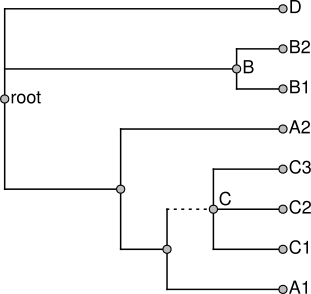
\includegraphics[scale=0.5]{Figures/fig1/synth1-no-is-shaded}}
\hfill{}\subfloat[Synthesis Tree (\emph{incertae sedis} aware)]{\includegraphics[scale=0.5]{Figures/fig1/synth1-shaded}}

\caption{\label{fig:Handling-incertae-sedis}Handling \emph{incertae sedis
}taxa recovers additional edges and taxon names.
Supertree construction on input tree (a) and taxonomy tree (b) with \emph{incertae sedis}
clade $C$ leads to synthesis tree (c) if \emph{incertae sedis} annotations are
ignored, but to synthesis tree (d) if \emph{incertae sedis} annotations are respected.
The tree in (d) recovers taxon names $AB$ and $A$, as well as the edge to clade $AB$
that groups $A$ and $B$. Taxon names and edges that are conditional on handling
\emph{incertae sedis} are shaded grey. \mthcomment{We could use triangle to indicate that $D$ and $B$ could be leaves or clades.}
}

\end{figure}

\subsection{A naive semantics: consequences of ignoring the annotation}

The most straightforward approach for increasing the taxonomic completeness of
the supertree is simply to no longer prune taxa from $\taxonomy$ because they are flagged
as \emph{incertae sedis}, and then run the rest of the pipeline of
\citet{redelings2017supertree} unaltered.  Before we propose a semantics of
\emph{incertae sedis}, it is worth pointing out what this naive semantics is lacking.

This approach incorrectly treats the intrusion of an \emph{incertae sedis} taxon
into a sibling taxon as a conflicting with monophyly of the sibling taxon. For
example, in Fig. \ref{fig:Handling-incertae-sedis}, the placement of the
\emph{incertae sedis} taxon $C$ within $A$ and $AB$ is considered
to contradict the monophyly of $A$ and $AB$ and thus to conflict with those taxa.
This has three main effects.  These effects are illustrated in the difference
between the synthesis tree in Fig. \ref{fig:Handling-incertae-sedis}c, which
ignores \emph{incertae sedis} annotations, and the synthesis tree in Fig.
\ref{fig:Handling-incertae-sedis}d, which respects them.

First, the naive approach results in a less-resolved tree.  While input trees are
free to place \emph{incertae sedis} taxa within a sibling, the naive approach
interprets this placement as conflict with the sibling.  Since the taxonomy
is ranked below all input trees, conflict is always resolved in favor of the
input trees, and so the sibling in the taxonomy is removed from the synthesis
tree.  For example, in the synthesis tree in Fig.
\ref{fig:Handling-incertae-sedis}c, the placement of taxon $C$ in group $AB$ is
interpreted as a rejection of the monophyly of $AB$. The edge leading to $AB$ is
therefore not incorporated into the synthesis tree.  In contrast, the synthesis
tree in Fig. \ref{fig:Handling-incertae-sedis}d that does not reject the
monophyly of $AB$ retains the grouping of $A$ and $B$.

Second, the naive approach results in the removal of clade names for all clades that
have an \emph{incertae sedis} taxon placed within them.  For example, in Fig.
\ref{fig:Handling-incertae-sedis}c the names for the clades $A$ and $AB$ are lost.

Third, the naive approach cannot use information from phylogenies to resolve the
location of uncertain taxa.  For example, the synthesis tree in
\ref{fig:Handling-incertae-sedis}c has lost the label for $A$, and so does not
allow us to note that $C$ has been placed within $A$.  In contrast, the synthesis
tree in Fig. \ref{fig:Handling-incertae-sedis}d retains the label for $A$, which
allows us to resolve taxonomic uncertainty by inferring that $C$ has been placed
within $A$.

\section{\label{sec:Semantics-of-incertae}Semantics of \emph{incertae
sedis} taxa}

\subsection{Goals for an \emph{incertae sedis} semantics}

In order to incorporate \emph{incertae sedis }taxa into a supertree
analyses, we must arrive at an operational definition of the meaning
of the \emph{incertae sedis} label.
The core meaning of the phrase is
that the annotated taxon may actually be a member of one of the taxa
that appear as siblings to it in the heirarchical representation of
the taxonomy.
In the most expansive interpretation, the author of the
taxonomy is stating that the \emph{incertae sedis} taxon could be
placed anywhere inside one of the sibling taxa or their descendants.
However, frequently only a subset of the possible placement points
would be viewed as plausible.

We seek a semantics for supertrees with \emph{incertae sedis }taxa
that satisfy the following properties:
\begin{enumerate}
    \item An \emph{incertae sedis} node may intrude into its siblings and their descendants without conflict.
    \item An \emph{incertae sedis} node has an unrestricted range within the descendants of its sibling taxa.
    \item The semantics of an \emph{incertae sedis} node does not depend on additional information such as taxon ranks, but only on the taxonomy tree.
    \item The semantics is based on deriving a rooted (partial) split for each branch of the taxonomy.
      % These could be goals, but maybe discuss them as side-effects:
      % Side effect #1. Don't interdigitate
      % Side effect #2. Allow placing A next to B, and then placing B within A. (See Fig. 6)
\end{enumerate}

\subsection{Terminology for rooted splits}

The rooted split associated with taxonomy node $n$ serves to determine both when $n$ is in conflict
with an input tree, and where to place the taxon name for clade $n$ on the synthesis tree.
% Removed mention of incertae sedis possibly affecting subproblem decomposition.  It
% actually doesn't but that is surprising, and therefore kind of a result.
% \paragraph{Definition of rooted splits}
As is typically done, we define rooted splits for each node by noting that
removing the edge connecting the node to its parent would produce two trees.
The leaf label sets of these trees partition the full leaf set $\mathcal{L}$ into two groups: the include
set $\mathcal{I}(n)$ which does not contain the root, and the exclude set $\mathcal{E}(n)$
which does contain the root. Such a split may be written
\[ \mathcal{I}(n)|\bullet\mathcal{E}(n).\]
where the $\bullet$ indicates the root. The include set is the set of labels for leaves that are
descendants of the node. The exclude set is the set of 
labels for leaves that are not descendants of that node.
The ``include set'' and ``exclude set'' of a ``rooted split'' used here are equivalent
    to the ``inside set'' and ``outside set'' of a ``$n$-taxon statement''
    \citep[\emph{sensu}][]{Wilkinson1994}.

If no taxa are \emph{incertae sedis},
then the exclude set for a node is just the total tip set minus the include set
for the node: $\mathcal{E}(n)  =\mathcal{L}-\mathcal{I}(n)$.
%For a node $n$ on the tip-ward side of an edge $e$, we
%may also write $\mathcal{I}(n)$ for $\mathcal{I}(e)$, and $\mathcal{E}(n)$ for $\mathcal{E}(e)$.
For any two rooted splits $A=A_{1}|\bullet A_{2}$
and $B=B_{1}|\bullet B_{2}$ , we say that $A$ \emph{displays }$B$ if $B_{1}\subseteq A_{1}$ and $B_{2}\subseteq A_{2}$.

Note that when a taxon rooted at node $n$ is not marked as \emph{incertae sedis},
then the leaf labels that are descendants of $n$ will be in the include set for
$n$ and all its ancestors and will be in the exclude set for all other nodes.

\paragraph{Equivalence of a taxonomy tree and a list of rooted splits}

Note that, for the purposes of the supertree method, all of the information from
the taxonomic tree is contained in the set of rooted splits. Thus, one could
imagine replacing that taxonomy, $\taxonomy_{p}$, with a set of rooted splits $\mathcal{R}(\taxonomy_{p})$ such that
each edge in $\taxonomy_{p}$ is encoded in one split in $\mathcal{R}(\taxonomy_{p})$. If the order of trees is set
to be: $\mathcal{R}(\taxonomy_{p})=\mathcal{Z}(\taxonomy_{p}) + 
\mathcal{Y}(\taxonomy_{p})$, then using $\mathcal{R}(\taxonomy_{p})$ in place of $\taxonomy_{p}$ in the supertree
algorithm would produce the same output.

\paragraph{Equivalence of rooted split definitions and phylogenetic definitions of names}
In terms of phylogenetic nomenclature the supertree pipeline acts as if the
taxonomy defines a conditional node-based name \citep[see][]{deQueiroz2013} for each
higher taxon.
So for the name labeling node $n$ in the taxonomic
tree, the operational definition would be: ``the clade defined by the most recent
common ancestor (MRCA) of $\mathcal{I}(n)$ as long as that MRCA is not an ancestor of
$\mathcal{E}(n)$.''
OTT is not based on a set of explicitly defined phylogenetic name definitions.
In many contexts, a branch-based definition for $n$ (``the clade by all of the taxa more
closely related to all fo them members of $\mathcal{I}(n)$ than to any member of
$\mathcal{E}(n)$, if such a clade exists'') would result in similar behavior
during the tree construction. 
An exception to this (discussed below) arises in the step of assigning names to the 
    supertree.

\paragraph{Equivalence of rooted split definitions with character encodings}
Representing a split in a tree by a character is the basis of one of the oldest
supertree methods: matrix representation with parsimony \citep[MRP, see][]{Baum1992,Ragan1992}.
In the rooted form of such an approach, character state 1 is used for tips that are
descendants of a internal node in an input tree and 0 is used for other tips and for the root.
Partial splits, such as those caused by \emph{incertae sedis} annotations, are naturally encoded by
encoding missing labels in a split as missing data in the corresponding character
(typically denoted with the `?' symbol in a matrix).

A rooted split is equivalent to the corresponding character in a matrix representation in the
sense that each can be treated as a condition that each tree may or may not satisfy.  A tree satisfies
a split if there a branch which divides include and exclude group when cut.  A tree satisfies the
corresponding character in a matrix representation if the character has a parsimony score of $1$ on the tree.  This equivalence is illustrated in Figure \ref{fig:Handling-incertae-sedis-mrp}.  Thus the taxonomy shown in Figure \ref{fig:Handling-incertae-sedis}b could be represented in terms of the splits
in Figure \ref{fig:Handling-incertae-sedis-mrp}a or the characters in Figure \ref{fig:Handling-incertae-sedis-mrp}b.  In the naive treatment of ignoring the \emph{incertae sedis} annotation, the `?' characters in the row for taxa $C1$ and $C2$ would be replaced with 0's.  Equivalently, the naive interpretation would add $C1$ and $C2$ to the exclude set for the $A$ and $AB$ splits.

   \begin{figure}
     \subfloat[Split representation]{
\noindent\begin{minipage}[t]{0.45\columnwidth}%
\begin{align*}
C & =C1\,C2\,\phantom{B\,}|\bullet\,A1\,A2\,B\,D\\
A & =A1\,A1\,\phantom{B\,}|\bullet\,B\,D\\
AB & =A1\,A2\,B\,|\bullet\,D
\end{align*}
%
\end{minipage}

}
     \subfloat[Matrix representation]{
         \begin{tabular}{|r|p{2em}|p{2em}|p{2em}|p{2em}|}
           \hline
           & \multicolumn{3}{|c|}{Character/clade label} \\
           leaves & C & AB & A \\
           \hline
           $A1$       & 0 & 1 & 1 \\
           $A2$       & 0 & 1 & 1 \\
           $B$        & 0 & 1 & 0 \\
           $C1$       & 1 & ? & ? \\
           $C2$       & 1 & ? & ? \\
           $D$      & 0 & 0 & 0 \\
           (root)     & 0 & 0 & 0 \\
           \hline
         \end{tabular}
}
       \caption{\label{fig:Handling-incertae-sedis-mrp} Rooted splits have an equivalent matrix encoding.
        (a) Rooted splits for an \emph{incertae sedis} interpretation of the taxonomy shown in  Figure \ref{fig:Handling-incertae-sedis}b. (b) The equivalent matrix representation. The root is coded as a special leaf. Split C is a full split, because it mentions all labels.  Splits A and AB are partial splits, and therefore have missing labels in the left panel, and '?' in the right panel.
       }

\end{figure}


\subsection{Split-based semantics for \emph{incertae sedis} taxa}

An \emph{incertae sedis} taxon $n$ differs from a normal taxon because it can be
placed as a descendant of some set of taxa without invalidating these taxa.
We will use $\mathcal{P}_n$ to denote this set of taxa which are {\emph{potential}} 
ancestors for \emph{incertae sedis} taxon $n$.
Note that this is distinct from the taxa that are ancestral to $n$ in the taxonomy;
    those are taxa which must contain all of the descandants of $n$.
The effect of the \emph{incertae sedis} annotation of taxon $n$ is
    to simply remove $\mathcal{I}(n)$ from the exclude set for each $p\in\mathcal{P}_n$.
The include sets of these splits remain unchanged, but the exclude sets may be reduced
\emph{incertae sedis} taxa to intrude.
Such a split does
not mention the complete set of tip labels $\mathcal{L}$ and is therefore called a
`partial split'', as opposed to a ``full split'' that contains the entirely of $\mathcal{L}$.

When considering \emph{incertae sedis} annotations, the taxonomy is still comprehensive 
if we include the degenerate grouping for the base
    node $\rho$ which has $\mathcal{I}(\rho) = \mathcal{L}$ and $\mathcal{E}(\rho) = \emptyset$,
    but many of the taxonomic nodes will correspond to partial splits.
Thus, when interpreted correctly the \emph{incertae sedis} 
annotations are reducing the amount of information that the taxonomy brings to
the supertree problem.


%  of any of its siblings.
% Thus, annotating $n$ as
% \emph{incertae sedis} really modifies the meanings of the taxanomic statements (rooted splits)
% of other
% that of the siblings of $n$ and all taxonomic nodes that descend from those siblings.
%  so that they
% no longer exclude $n$.
% %In terms of rooted splits, we can represent this lack of
% %   exclusion by omitting taxa from the exclude set for a node.
% % We seek to define modified splits for each branch of the taxonomy tree.
%  into their sibling taxa.
% % Therefore, a semantics can be given simply in terms of the exclude set for each taxonomy node.


\subsection{Unrestricted range and ignoring additional information}
In principle, an \emph{incertae sedis} taxon $n$ could carry with it additional
    information that indicates which specific points within the taxonomic tree
    it could attach.
Unfortunately, reliable information about the range of valid attachment points
for each \emph{incertae sedis} taxon is lacking in OTT and most other large-scale
taxonomies.
Constructing a range for each incertae sedis taxon relies on detailed
readings of character argumentation (which is lacking in OTT) or rank-based
information (which is frequently untrustworthy in OTT). Thus, here we pursue
an approach of ascribing a meaning to the \emph{incertae sedis} label which
attempts to capture the core of the idea that it articulates, but which can be
applied automatically across the taxonomy without additional information.


Specifically, the methods described here only consider cases in which 
    $\mathcal{P}_n$ can be determined from the structure of the tree.
Our method takes $\mathcal{P}_n$ to be the set of nodes that
    are in the taxonomic subtrees rooted at the sibling taxa of \emph{incertae sedis} taxon $n$.
This allows us to encode the exclude set of some node $x$ efficiently by sweeping
    over the tree from root to tip.
If $\mathcal{S}(x)$ is the set of siblings of $x$ and $p(x)$ is the parent of $x$, then
the naive approach of ignoring the \emph{incertae sedis}  annotation amounts to setting
    the exclude set as:
\begin{align}
    \mathcal{E}(x) = \mathcal{E}(p(x)) \cup \left\{ \bigcup_{s\in \mathcal{S}(x)} \mathcal{I}(s) \right\}
    \label{eq:exsetformonea-traditional}
\end{align}
with $\mathcal{E}(\rho) = \emptyset$ for the root of the taxonomic tree.

If we treat the  \emph{incertae sedis} annotation as an indication that the 
    \emph{incertae sedis} taxon $x$ can be placed in any of its sister taxa, then
    we let $\mathcal{Q}(x)$ denote the set of siblings of $x$ that are not
    flagged as being \emph{incertae sedis} and we define the exclude set as:
\begin{align}
    \mathcal{E}(x) = \mathcal{E}(p(x)) \cup \left\{ \bigcup_{s\in \mathcal{Q}(x)} \mathcal{I}(s)\right\}
    \label{eq:exsetformonea}
\end{align}
We will refer to this interpretation of the \emph{incertae sedis} annotation as ``unrestricted
    intrusion'' semantics.

%If $\mathcal{P}$ is the set of taxa that are potential ancestors for \emph{incertae
%  sedis} taxon $x$, then we may simply remove the descendants of $x$ from the exclude
%  set for each $p\in\mathcal{P}$.  Such an approach would require that the path from $x$ to $p$
%  go through only other potential ancestors.

% Supporting more precise information about $\mathcal{P}_n$  for each \emph{incertae sedis}
%    taxon $n$ is an important future direction to be explored.
% For example, a genus
% might be characterized as \emph{incertae sedis} at the level of the subfamily.
% Thus, it could be placed inside any of the hypothesized sub-families, or within
% its own subfamily, but it would be unexpected for it to be placed inside one of
% the other genera.


% In order to determine how the exclude sets should be modified to account for
% \emph{incertae sedis} taxa, we first attempt to express the unmodified exclude
% sets in a helpful way.  We note that a node $n$ ordinarily excludes the
% descendants of $\mathcal{I}(s)$ for all of its siblings, as well as the siblings
% of all of its ancestors.  This leads to the following equation:
% \begin{align}
% \mathcal{E}(n) & = \mathcal{L} - \mathcal{I}(n)\nonumber\\
%  & =\left[\mathcal{I}(s)\big|a\in n+ancestors(n),s\in siblings(a)\right]\nonumber\\
%  & =\left[\mathcal{I}(s)\big|s\in siblings(n)\right]\cup\left[\mathcal{I}(s)\big|a\in ancestors(n),s\in siblings(a)\right]\nonumber\\
%  & =\left[\mathcal{I}(s)\big|s\in siblings(n)\right]\cup\mathcal{E}(parent(n)).\label{eq:exsetformonea-traditional}
% \end{align}

% When modifying the exclude set for a node $n$, we seek to find all the \emph{incertae
% sedis} taxa that may intrude into it. It turns out that the incertae sedis taxa that
% might intrude are just the \emph{incertae sedis} siblings of $n$ and all of its ancestors.
% \begin{align}
% \mathcal{E}(n) & =
%     \left[\mathcal{I}(s)\big|a\in n+ancestors(n),s\in siblings(a),s\text{ not \emph{incertae sedis}}\right]\nonumber\\
% & =\left[\mathcal{I}(s)\big|s\in siblings(n),s\text{ not \emph{incertae sedis}}\right]\cup\nonumber\\
% & \,\,\,\,\,\,\,\,\,\,\,\,\left[\mathcal{I}(s)\big|a\in ancestors(n),s\in siblings(a),s\text{ not \emph{incertae sedis}}\right]\nonumber\\
% & =\left[\mathcal{I}(s)\big|s\in siblings(n),s\text{ not \emph{incertae sedis}}\right]\cup\mathcal{E}(parent(n)).\label{eq:exsetformonea}
% \end{align}
% This formula allows us to compute exclude sets via a pre-order traversal on the
% taxonomy tree with the exclude set for the root node defined to be $\emptyset$. 


\subsection{Naming }

\begin{figure}
\hfill{}\subfloat[Taxonomy tree]{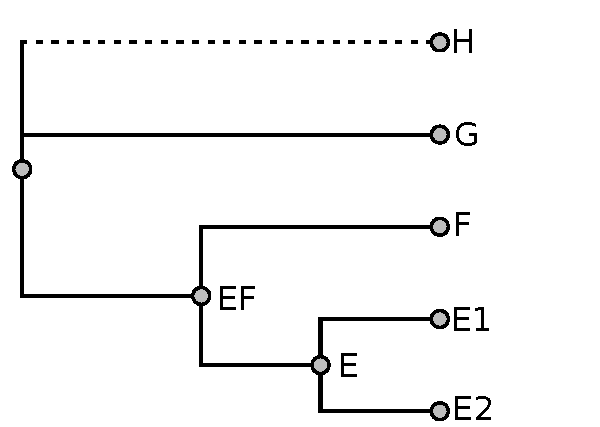
\includegraphics[scale=0.5]{Figures/name1nodes2/tax-shaded}}
\hfill{}\subfloat[Solution tree]{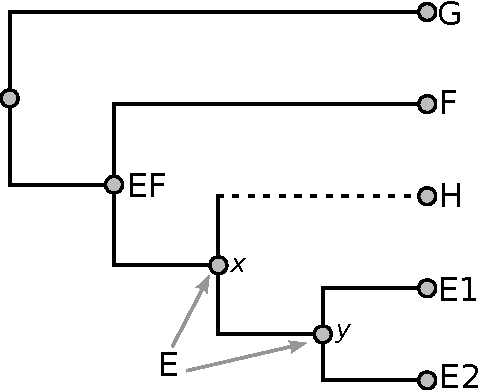
\includegraphics[scale=0.5]{Figures/name1nodes2/solution-shaded}}
\hfill{}
\caption{\label{fig:One-name-can}One name can be consistent with multiple nodes.}
\end{figure}

After constructing a supertree, tip nodes already have names in \emph{$\mathcal{L}$}.
However, we still need to assign higher taxon names to internal supertree nodes
based on the taxonomy tree in the problem. Each taxon name $n$ corresponds to a
split $S(n)=S(n)_{1}|\bullet S(n)_{2}$ on the corresponding branch of the taxonomy tree. Without
\emph{incertae sedis}, such splits are always of the form $S(n)_{1}|\bullet\mathcal{L}-S(n)_{1}$, but
with \emph{incertae sedis} taxa $S_{2}(n)$ may be smaller than $\mathcal{L}-S(n)_{1}$.

Without \emph{incertae sedis}, each name applies to at most one node, and each
node can take at most one name, with the exception of monotypic taxa. Thus, we
may simply search the solution tree for a node that has the same cluster $S(n)_{1}$
and apply the name $n$ to that node.

However, in the \emph{incertae sedis} framework, it is possible for one name to
apply to multiple nodes. For example, in Figure \ref{fig:One-name-can}b, the
name $E$ can apply to nodes $x$ and $y$. Here the name $E$ corresponds to the split
$E1\,E2\,|\bullet F\,G$, leaving $H$ out of the definition since $H$ is \emph{incertae sedis}. 
The two nodes $x$
and $y$ display the splits $E1\,E2\,|\bullet F\,G\,H$ and $E1\,E2\,H|\bullet
F\,G$ respectively, and both
of these splits display the split $E1\,E2\,|\bullet F\,G$, so the name $E$ can apply to both
$x$ and $y$. 
This cannot happen when the rooted splits that correspond to a taxonomic name
    are generated without\emph{ incertae sedis} taxa except at
monotypic nodes.

This situation is the result of the fact that it is not clear whether the names
    in the taxonomic tree should be treated as node-based or branch-based
    phylogenetic defintions.
A node-based definition of $E$ would be ``the clade rooted at the MRCA of $E1$ and $E2$ as long as it is not
    the ancestor of $F$ or $G$''; this would correspond to node $y$ in the solution
    depicted in figure Figure \ref{fig:One-name-can}b.
The branch-based definition would take the form ``The clade containing all lineages more closely related to 
   $E1$ and $E2$ than to either $F$ or $G$, if such a clade exists''; this definition
   would include node $x$ and the lineage connecting it to its parent.
The ambiguity arises because both definitions refer to the same node in the taxonomy,
    so it is unclear which is a preferable way to define the taxon concept of $E$.

When faced with a choice about where to place a name, our
solution is to find the most tip-ward node where the name can apply and attach
the name to this node.
This corresponds to using a node-based definition of the taxonomic names.
The result of this naming choice is that the algorithm is conservative with respect
    to when the \emph{incertae sedis} taxa should be placed within another named
    taxon.

Note that the intrusion of an \emph{incertae sedis} taxon within another taxon does not
    always lead to ambiguity in which node should be named. 
For example, $H$ is placed inside taxon $EF$ in Figure \ref{fig:One-name-can}, but the
    the name $EF$ only applies to one node in the solution tree.

\begin{figure}
\hfill{}\subfloat[Taxonomy tree]{\includegraphics[scale=0.5]{Figures/names2nodes1/tax-shaded}}
\hfill{}\subfloat[Solution tree]{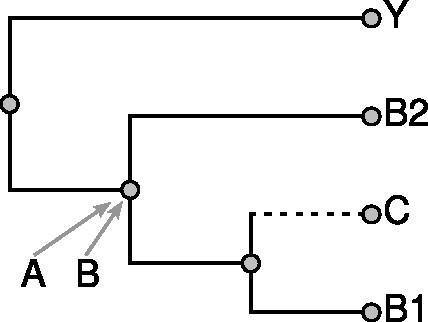
\includegraphics[scale=0.5]{Figures/names2nodes1/synth-shaded}}
\hfill{}\subfloat[Solution tree]{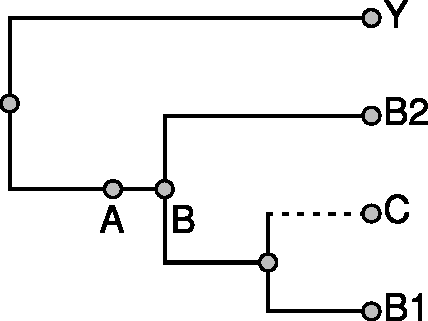
\includegraphics[scale=0.5]{Figures/names2nodes1/solution2-shaded}}
\hfill{}
\caption{\label{fig:Multiple-names-can}Multiple names can apply to a single node.}
\end{figure}

It is also possible for multiple names to apply to a single node. For example,
in Figure \ref{fig:Multiple-names-can}a, the taxon $M$ corresponds to the split
$L1\,L2\,K\,|\bullet\,J$, and its child taxon $L$ corresponds to the split $L1\,L2\,|\bullet\,Y$.
The edge leading to $M$ is consistent with the split for $L$, but the name $L$ is
applied to the node with the smallest include group.
However, in the
solution tree (Fig. \ref{fig:Multiple-names-can}b), there is is only node for
both names $M$ and $L$ to apply to.
This kind of situation arises when a taxon
becomes monotypic after its \emph{incertae sedis} children are placed elsewhere.
For such cases, we can address this synonymy by (i) selecting a taxon at the
node that is ancestral to all other taxa and (ii) moving this taxon to a
newly-introduced out-degree-1 parent.  For example, $M$ is moved to an
out-degree-1 parent in Fig. \ref{fig:Multiple-names-can}c.
We repeatedly perform
this procedure until no taxon at the node is the parent of all taxa.


However, there are cases where thus procedure does not result in one name per
node.  This case can occur, for example, when two \emph{incertae sedis} siblings are 
``inter-digitated'', or  combined into a single clade in such a way that their
members cannot be separated.  When the members of the two clades share the same
MRCA, as in Fig. \ref{fig:interdigitation}, then the names for both clades
apply to the same node.  However, in this case, neither name is ancestral to
the other, and the previous solution does not apply.
In such cases, we treat all applicable names as synonyms for the node.
\mthcomment{Need to verify that the namer records this situation as synonyms, as it should!}
\bdrcomment{I assume this is not linked to publication}

\begin{figure}
\hfill{}\subfloat[Taxonomy tree]{\includegraphics[scale=0.5]{Figures/is-interdigitation/tax-shaded}}
\hfill{}\subfloat[Solution tree]{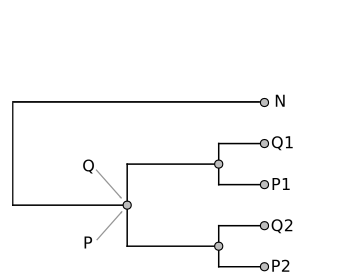
\includegraphics[scale=0.5]{Figures/is-interdigitation/synth-shaded}}
\hfill{}
\caption{\label{fig:interdigitation}Interdigitation of \emph{incertae sedis} siblings.  Here the names $P$ and $Q$ apply to the same node on the solution tree, but neither is ancestral to the other on the taxonomy.}
\end{figure}



\subsection{Taxonomic revision}\label{subsec:Placement}

After we have attached taxon names to the synthesis tree, we would
like to interpret the position of these names in terms of placing
\emph{incertae sedis }taxa in a revised taxonomy.
This would allow us
to interpret the synthesis tree as saying that phylogenetic
information has (for example) placed genus A within family B, or
perhaps outside of all named families.
The simplest approach to
placement involves noting whenever a taxon $B$ is a descendant of a
taxon $A$ on the named synthesis tree but not the taxonomy tree.
For
example, in Figure \ref{fig:Handling-incertae-sedis}, taxon $C$ is a
descendant of taxon $A$ in the synthetic tree 
(Fig.\ref{fig:Handling-incertae-sedis}d), but not the taxonomy 
(Fig.\ref{fig:Handling-incertae-sedis}b).
Thus, we could say that the synthetic tree places
$C$ within $A$. 
%Furthermore, the synthetic tree additionally places
% $C$ within $AB$.

In general, after naming the clades in the supertree, the
    taxonomic placement of an \emph{incertae sedis} taxon
    can be detected if the most tip-ward named ancestor of
    the clade in the supertree was not an ancestor in the
    taxonomic tree.
Note that if an \emph{incertae sedis} taxon is broken
    during the supertree algorithm, it can be ambiguous whether
    or not all of the members should be placed in a new
    parent taxon.
See, for example, Figure \ref{fig:Broken-incertae-sedis}.
Here taxon $T1$ is an descendant of $R$ in the
synthesis tree, but not the taxonomy.
Thus $T1$ is placed within $R$; taxon
 $T2$ is similarly placed with in $R$.
$T3$ is not mentioned in either input tree, and the 
    only tree that speaks to its placement is the taxonomic input.
However, the taxon $T$ cannot be monophyletic based on the
     two input trees.
Thus the correct placement of $T3$ is uncertain.

The ambiguity of where to place $T3$ can also be compared to the
    behavior of maximum compatibility tree estimation and parsimony.
The matrix representation context the taxonomic tree's
    character representation of taxon $T$ would include $T1$, $T2$ and $T3$
    all being assigned state 1 and all of the other leaves being assigned 
    state 0.
This character is not compatible with the solution tree. 
The compatability approach would be to conclude that the character encoding 
    that taxon was incorrect and should be ignored.
Since, no other character speaks to the position of $T3$, it would fall to being
    a child of the root of the tree.
In a similar result, the BUILD algorithm would place $T3$ as a child of the root.

In a parsimony view, while the character cannot be mapped onto the solution in
    a homoplasy-free manner, one might hope that the character data that the
    taxonomy was based on was not completely unreliable.
Placing of $T3$ as either sister to $T1$ or $T2$ could explain the character
    representation of taxon $T$ with only two acquisitions of the state 1.
Other placements of $T3$ would require at least three 0 to 1 changes (or a reversion
    to state 0)l
Placing $T3$ at the MRCA 
    of the other members of $T$ corresponds
    to handling of ``rogue'' taxa in an Adams consensus method of the two
    most parsimonious placements of $T3$ under an irreversible parsimony model.



% We note that the MRCA of $R$ and $T1$ in
% the taxonomy is the root node, and the path to the ch from $R$ is
% $R\to RS\to root$, while the path to the MRCA from $T1$ is $T1\to T\to
% root$.
% Here the additional node $RS$ on the path to the MRCA from $R$
% indicates that $T1$ is placed within $RS$ as well as $R$.
% In contrast,
% the additional node $T$ on the path to the MRCA indicates that $T1$ is
% a broken \emph{incertae sedis} taxon.
% Thus we may consider an
% algorithm that, for each taxon $S$ on the synthesis tree, finds the
% closest ancestral taxon $A$, and checks if $A$ is an ancestor of $B$
% on the taxonomy.
% If not, we compute the paths $A\to A_{1}\to\ldots\to
% MRCA(A,B)$ and $B\to B_{1}\to\ldots\to MRCA(A,B)$.

\begin{figure}
\hfill{}\subfloat[Input tree \#1]{\includegraphics[scale=0.5]{Figures/is-clade/tree1-shaded}

}\hfill{}\subfloat[Input tree \#2]{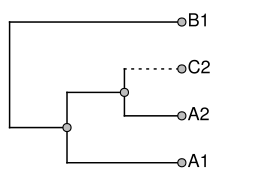
\includegraphics[scale=0.5]{Figures/is-clade/tree3-shaded}

}\hfill{}

\hfill{}\subfloat[Taxonomy]{\includegraphics[scale=0.5]{Figures/is-clade/tax-shaded}

}\hfill{}\subfloat[Synthesis Tree \#1]{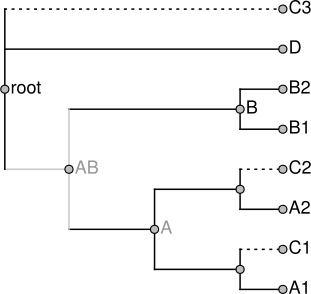
\includegraphics[scale=0.5]{Figures/is-clade/synth2-shaded}

}\hfill{}

\caption{\label{fig:Broken-incertae-sedis} \emph{Incertae sedis} clade $T$
broken by conflicting placement.
Input trees (a) and (b) conflict
in the placement of taxa in $T$.
The synthesis supertree (d) places
places $T1$ and $T2$ separately within $R$.
The BUILD algorithm would place the unsampled taxon $T3$ at the
root of the tree, while our unprune operation implemented to 
handle taxonomy-only taxa would place $T3$ as a child of the MRCA
of the other members of $T$, as pictured in (d).
}

\end{figure}

\subsection{Ambiguity of imputed taxonomic characters}
It is tempting to view the matrix representation of the taxonomic tree
    as an encoding of the presence, absence, and uncertainty about
    suites of synapomorphies which allow us to diagnose a taxon.
Clearly by simply representing the taxonomic tree, we will not be
    able to recover the identity or even the number of characters that
    a taxonomist might have used when classifying the organisms in question.
Nevertheless, one might hope that a matrix representation of a taxonomy (such
    as the matrix in Figure \ref{fig:Handling-incertae-sedis-mrp} as a 
    representation of Figure \ref{fig:Handling-incertae-sedis}b) has a unique, uncontroversial 
    association with the taxonomic tree.

The rules for associated leaves in $\mathcal{I}(n)$ with state 1, leaves
     in $\mathcal{E}(n)$, and other leaves with the missing data symbol 
     do allow to encode the taxon $n$ in a taxonomic tree unambiguously.
However, these are not the only set of rules for generating a character matrix
    representation that would cause the taxonomic tree allows the characters to
    be mapped without homoplasy.
For example consider the case of the taxonomy shown in Figure \ref{fig:Placing-one-incertae}a.
Either of the two matrices shown in \ref{fig:Placing-one-incertae-MRP} could encode this
    taxonomy along with its \emph{incertae sedis} interpretation.
The matrix in Figure \ref{fig:Placing-one-incertae-MRP}a would result in the 
    taxon $V$ not being named in the supertree shown in Figure \ref{fig:Placing-one-incertae}b,
    while the matrix shown in Figure \ref{fig:Placing-one-incertae-MRP}b would lead
    to $V$ being named.
Thus, accurately
    honors the input taxonomic content we would need more taxonomic information
    than simply a hierarchy and knowledge of which taxa can float more tipward.

Note that this example also presents a challenge for iterative supertree building and refinement
    of the taxonomy without retention of additional information.
Consider the case, in which there are two phylogenetic inputs along with the taxonomy from
    tree Figure \ref{fig:Placing-one-incertae}b with the first phylogeny, $T_1$, providing the single
    rooted split: $V1\,X \mid \bullet\,U$ and the second phylogeny, $T_2$ providing the 
    rooted split: $W\, V1 \mid \bullet\,V2$.
If the supertree pipeline were run with just the taxonomy and and $T_1$ as inputs, then the supertree
    would be the tree shown in Figure \ref{fig:Placing-one-incertae}c.
One might hope that using that tree as the revised taxonomy and then adding the split from $T_2$ in
    a subsequent analysis would result in the same tree as if $T_1$ and $T_2$ to the original taxonomy.
While the topology for the final tree in either order of analyses would indeed be the tree shown in 
    Figure \ref{fig:Placing-one-incertae}b, the decision about whether or not to name $V$ would differ.
Our handling of \emph{incertae sedis} in the original taxonomy via rooted partial splits
    would encode the taxonomic definitions in the manner depicted in Figure \ref{fig:Placing-one-incertae-MRP}a,
    but the encoding of the revised taxonomy in Figure \ref{fig:Placing-one-incertae}c would result
    in an altered definition of taxon $V$, as shown in \ref{fig:Placing-one-incertae-MRP}c.
As expected, in the encoding of the revised taxonomy, the definition of $WX$ has been altered to reflect the
    fact $T_1$ placed $V$ inside $WX$.
Perhaps, unexpected is the fact that storing the revised taxonomy with an \emph{incertae sedis} annotation
    and then reprocessing the taxonomy using our rooted partial splits approach would also shift
    the definition of $V$ from a taxon that must exclude $W$ to one that may include $W$.


\begin{figure}
%\subfloat[Input tree \#1]{\includegraphics[scale=0.5]{Figures/is-within-is/tree1\lyxdot tre}}
\subfloat[Taxonomy]{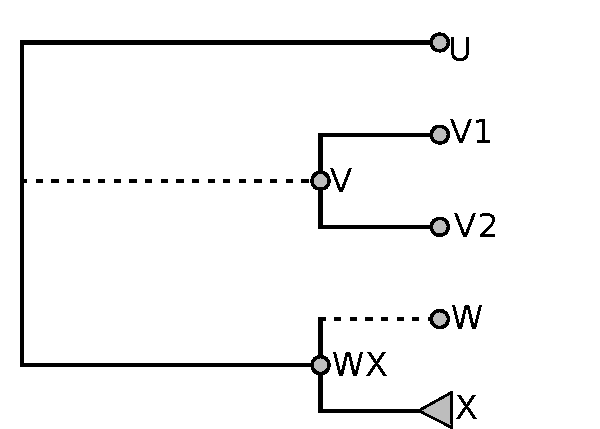
\includegraphics[scale=0.5]{Figures/is-within-is/tax-shaded}
}
\subfloat[Final supertree]{\includegraphics[scale=0.5]{Figures/is-within-is/synth1-shaded}
}
\subfloat[Possible intermediate]{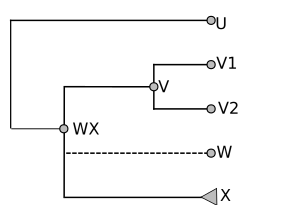
\includegraphics[scale=0.5]{Figures/is-within-is/intermed-shaded}
}

\caption{\label{fig:Placing-one-incertae}
One \emph{incertae sedis} group ($W$) being placed within another ($V$), with possible
loss of the taxon $V$.}
\end{figure}

\begin{figure}
%\subfloat[Input tree \#1]{\includegraphics[scale=0.5]{Figures/is-within-is/tree1\lyxdot tre}}
\subfloat[maximally scored]{
    \begin{tabular}{|r|p{2em}|p{2em}|}
\hline
& \multicolumn{2}{|c|}{Character} \\
taxa & $V$ & $WX$  \\
\hline
$U$  & 0 & 0  \\
$V1$ & 1 & ?  \\
$V2$ & 1 & ?  \\
$W$  & 0 & 1  \\
$X$  & 0 & 1 \\
\hline
\end{tabular}
}\hfill{}
\subfloat[less informative]{
    \begin{tabular}{|r|p{2em}|p{2em}|}
\hline
& \multicolumn{2}{|c|}{Character} \\
taxa & $V$ & $WX$  \\
\hline
$U$  & 0 & 0 \\
$V1$ & 1 & ? \\
$V2$ & 1 & ? \\
$W$  & ? & 1 \\
$X$  & 0 & 1 \\
\hline
\end{tabular}
}\hfill()
\subfloat[from revised taxonomy]{
    \begin{tabular}{|r|p{2em}|p{2em}|}
\hline
& \multicolumn{2}{|c|}{Character} \\
taxa & $V$ & $WX$  \\
\hline
$U$  & 0 & 0 \\
$V1$ & 1 & 1 \\
$V2$ & 1 & 1 \\
$W$  & ? & 1 \\
$X$  & 0 & 1 \\
\hline
\end{tabular}
}
\caption{\label{fig:Placing-one-incertae-MRP}
Panels (a) and (b) show two possible encodings that would support the $V$ and $WX$ branches and \emph{incertae sedis}
annotation shown in the taxonomy from in Figure \ref{fig:Placing-one-incertae}a.
The representations only vary in the scoring of leaf $W$ for character $V$. Panel (c) shows the information encoded by the tree in \ref{fig:Placing-one-incertae}c. }
\end{figure}


\section{Handling \emph{incertae sedis} taxa in the propinquity
pipeline}

In order to handle \emph{incertae sedis} taxa within propinquity \citep{redelings2017supertree}, we
must modify some of the stages of the propinquity pipeline.
Subproblem
decomposition must place \emph{incertae sedis} taxa in the correct
subproblem.
Subproblem files must indicate which taxa are \emph{incertae sedis}.
The subproblem solver must read this information, account for
\emph{incertae sedis} taxa when solving subproblems, and correctly
name taxa that have been modified by having \emph{incertae sedis} taxa
place inside them.
The unpruner must be aware of \emph{incertae sedis}
taxa.
Annotations of the tree must be aware of \emph{incertae sedis}
taxa so that it does not consider taxa broken when they have an
\emph{incertae sedis} taxon placed inside them.



% \newpage %TEMP

\begin{figure}
\subfloat[$\tau_{1}$]{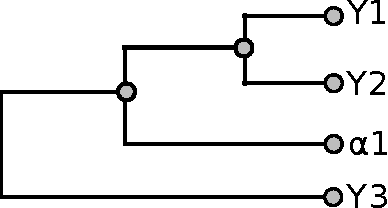
\includegraphics[scale=0.5]{Figures/decomp/tree1}
}\hfill{}
\subfloat[$\tau_{2}$]{
\includegraphics[scale=0.5]{Figures/decomp/tree2}
}\hfill{}
\subfloat[$\tau_{3}$]{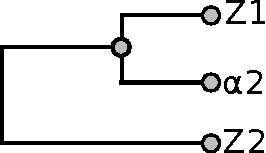
\includegraphics[scale=0.5]{Figures/decomp/tree3}
}\hfill{}
\subfloat[$\tau_{4}$]{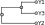
\includegraphics[scale=0.5]{Figures/decomp/tree4}
}

\subfloat[Taxonomy $\protect\taxonomy$]{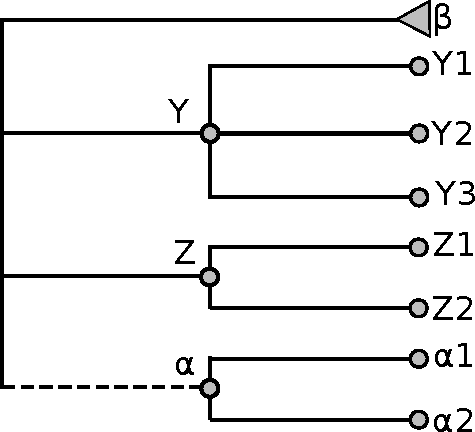
\includegraphics[scale=0.5]{Figures/decomp/tax}
}\hfill{}
\subfloat[$Y$ and $Z$ decomposition]{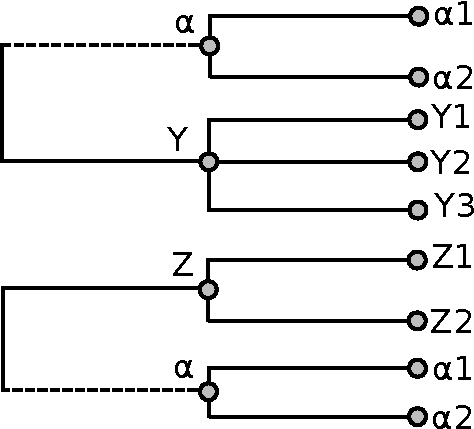
\includegraphics[scale=0.5]{Figures/decomp/decompRep}
}\hfill{}
\subfloat[Pruned $Y$ and $Z$ decomposition]{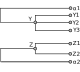
\includegraphics[scale=0.5]{Figures/decomp/decompPruned}
}


\caption{\label{fig:decomp} Four phylogenetic trees (a-d) an
example taxonomy (e) which are possible inputs to the propinquity supertree pipeline.
(f) shows the taxonomic component of the subproblem decompositions for taxa $Y$ and $Z$ subproblems 
that would result
from an unmodified pipeline with used $\tau_1$ and either $\tau_2$ or $\tau_3$ as the phylogenetic
inputs.
(g) shows a possible decomposition from a decomposition tool that avoids duplication of taxa.
}
\end{figure}





\subsection{Sub-problem decomposition}

The presence of \emph{incertae sedis }taxa poses a problem to sub-
problem decomposition, since taxonomy edges no longer completely
separate subproblems.
Instead, \emph{incertae sedis} taxa may attach
on either side of a taxonomy edge.
We seek to place \emph{incertae
sedis} taxa into subproblems in such a way that the subproblem solver
can perform the placement inside the subproblem.
This approach
postpones handling of conflict in \emph{incertae sedis} taxa to the
subproblem solver, where the problem is well formulated in terms of
splits.
However, it does have the effect of creating larger
subproblems.

Simply allowing the subproblem decomposer to recognize that intrusion
    of an \emph{incertae sedis} taxon does not contest the existence
    of a clade would be straightforward, but problems arise if the
    decomposer is not further altered.
Consider, for example, the inputs of the $\tau_1$, $\tau_2$, $\tau_3$, and the taxonomy
    shown in Figure \ref{fig:decomp}.
Because the taxon $\alpha$ is annotated as being \emph{incertae sedis}, 
    neither  $\tau_1$, $\tau_2$, nor $\tau_3$ contest the monophyly of 
    the taxa $Y$, $Z$, or $\alpha$.
This would lead to the taxonomic portion of both the $Y$ and $Z$ subproblems
    containing the taxonomy for $\alpha$, leading to the members of
    $\alpha$ occurring in two different subproblems (see Figure \ref{fig:decomp}f).
Solving and merging these problems would result in the duplication of $\alpha$ 
    in the supertree.


One could easily
    imagine a ``pruning decomposer'' that does not allow the same taxon to
    occur in more than one subproblem.
This approach would work in a straightforward way if the phylogenetic inputs were only $\tau_1$ and $\tau_3$,
    yielding the decomposition shown in Figure \ref{fig:decomp}g, but if
    both $\tau_1$ and $\tau_2$ were inputs the decomposer would have to
    resolve conflict about the placement of $\alpha_1$.
Implementing the behavior in the subproblem decomposition step would
    break the separation between the ``divide'' and ``conquer'' steps
    which is a key aspect of propinquity's current efficiency.

Even considering ranked phylogenetic inputs of $\tau_4$ then $\tau_1$ from
    Figure \ref{fig:decomp} reveal some difficulties.
In this case the inclusion of $\alpha$ within the taxon $Y$ in $\tau_1$ would
    cause $\alpha$ to be solved in the subproblem for $Y$.
If $\tau_4$ were ranked higher than $\tau_1$, then the grouping of $Y_1+Y_2+\alpha$ would
    not be permitted because they conflict with the split $Y_1\,Y_3 \mid \bullet\,Y_2$ from
    $\tau_4$.
Thus, $\alpha$ would be placed inside of $Y$ on the basis of a rooted split
    that is not displayed in the final tree.
While this is placement is permissible based on the \emph{incertae sedis} annotation of the
    taxonomy, a major goal of the propinquity pipeline is to make it
    easy for biologists to understand the cause of different groupings in the 
    supertree.
Allowing splits which are not displayed to determine the placement of groups runs counter to that goal.



We choose to solve these problems by merging any subproblems that an
\emph{incertae sedis} taxon might be placed in.
The simplest way to
achieve this is simply to regard any taxon that has an \emph{incertae
sedis }taxon placed within it as contested.
This results in marking
both $B$ and $C$ as contested edges in the example above.
In fact,
this is the current behaviour of the non-\emph{incertae-sedis} aware
subproblem decomposer.
One downside of this approach is that, an \emph{incertae sedis} taxon
    place in only one input tree, the clade it is placed in will be
    marked as contested even though none of the counterintuitive
    behaviors mentioned above would arise if we did not
    mark it as contested.



\subsection{Subproblem solution}

Our sub-problem solver naturally handles \emph{incertae sedis} taxa.
This is because we define the semantics of \emph{incertae sedis} taxa
in terms of partial splits, and our solver natively supports building
trees from partial splits through its use of the BUILD algorithm.
Handling \emph{incertae sedis} taxa thus requires loading incertae
sedis information and computing partial splits for \emph{incertae
sedis} taxa before solving a sub-problem.
After solving a sub-problem,
we must apply taxon names from the taxonomy tree to the sub-problem
solution tree.
The solution tree is considered to be a fixed tree and not
to have any \emph{incertae sedis} nodes, or any other forms of
uncertainty.


\subsubsection{Implementation: finding the node for a name}

To find the node for a name $n$, we find the MRCA of the cluster
$S_{1}(n)$.
If the MRCA excludes the entire exclude group $S_{2}(n)$
then the name applies to the MRCA; otherwise the taxon does not exist
on the tree.

\subsubsection{Implementation: handling name clashes}

When multiple names $N=\{n_{1},\ldots n_{N}\}$ map to the same
solution node $x$, then these names must satisfy some tree structure
on the taxonomy, such that $n_{1}<n_{2}$ if $n_{1}$ is a descendant of
$n_{2}$ in the taxonomy.
If it is possible to find a name $n_{max}$
that is the unique maximal element of $N$, then it is permissible to
\begin{enumerate}
    \item create a monotypic parent $p(x)$ of $x$, and
assign $n_{max}$ to $p(x)$ 
    \item continue handling name clashes at $x$
with the set of possible names reduced to $N-n_{max}$.

\end{enumerate}
However, its certainly possible that there might not be any such
$N_{max}$, in which case we could just choose a name for $x$ from $N$
(perhaps not an \emph{incertae sedis} name) and then record all the
other names as equivalents somewhere.

\bdrcomment{we might get this behavior in a
nice an automatic way if we create a single fake leaf for each
monotypic taxonomy node that holds the node's leaf label.}


\subsection{Annotation}

Annotation primarily involves running a conflict analysis between the
synthesis tree and each input tree.
Since neither tree has any
\emph{incertae sedis} taxa, the conflict algorithm does not need to
change.
Furthermore, if we allow \emph{incertae sedis} taxa that are
taxonomy-only to be annotated as \emph{incertae sedis} on the synth
tree, then such groups will not affect conflict with the input trees.
We would also like to allow running a conflict analysis between the
synthesis tree and the taxonomy tree.
However, naming the nodes
\emph{is} a (almost) run of conflict analysis on the taxonomy tree,
and this has already been done in a prior step.
So, the current
annotation procedure actually works as-is.

It would be nice to allow running conflict against the cleaned
taxonomy, though.
One way to do this would be to generated a ``placed
taxonomy'', with groups extended to include \emph{incertae sedis} taxa
that have been placed within them.
This would not require any updating
to the conflict-analysis code in the annotation step.

\section{Discussion}
\bdrcomment{This is slightly exaggerated in the sense that there might be other
  frameworks to incertae sedis taxa that do not require these exact moves.  Nonetheless,
  I think this is not just a ``review'', in the sense that any well-founded approach
  would have to work through all of these problems.  By working through them, we have
  navigated the paths that subsequent approaches will need to walk.

  I would argue that
  the fact that our solution seems relatively simple should be seen as a success, and not
  a sign that we haven't done enough work.  It often takes a lot of work to get a complex
  solution down to a simple solution.

  Additionally, the fact that we do not have
  a lot of ``results'', in the sense of (say) large number of higher-taxon names that
  are rescued by avoiding the naive approach, is a result of the fact that we didn't want
  to do the work to add more input phylogenies with incertae sedis tips that will cause
  problems.  We could always go back and try to get these ``results'', but the percieved value
  wasn't very high.  Also, the algorithm that we came up with is itself a ``result''.
}


This paper introduces the necessary concepts and methods for handling \emph{incertae sedis}
taxa in taxonomic supertrees.  We describe the goals of preserving internal edges,
preserving higher taxon names, and preserving the opportunity to revise the taxonomy
based on placement of \emph{incertae sedis} taxa.  In addition to explaining why
the naive approach to taxonomic supertrees that ignores incertae sedis taxa sacrifices
these three goals, we introduce a simple and satisfying way to achieve these goals
through defining rooted splits for taxonomy edges with reduced exclude sets.  We also
provide a simple and efficient recursion for computing these splits.

Despite the simplicity of our approach, some complexities and conceptual difficulties
remain.  While the correspondence of nodes and names is a simple one-to-one and onto
relationship without \emph{incertae sedis} taxa, when \emph{incertae sedis} taxa are
introduced, the relationship might be neither one-to-one (Figures \ref{fig:Multiple-names-can},\ref{fig:interdigitation}) nor onto (Figure \ref{fig:One-name-can}).
This necessitates putting more thought into the semantics of taxon names, including
whether names might become synonyms.  This may be considered a ``complexity''.

In addition, our attempt to define reduced exclude sets for taxonomy splits yields
a semantics that is not the only concievable semantics for \emph{incertae sedis}
taxa (Figure \ref{fig:Placing-one-incertae}).  It allows \emph{incertae sedis} siblings to inter-digitate
(Figure \ref{fig:interdigitation}), which might be a surprising result to the taxonomist.  Furthermore,
in what might seem a lack of consistency, it does \emph{not} allow \emph{incertae sedis}
taxa to intrude into each other if they become siblings through the result of
placement, as is the case for taxa W and V in Figure \ref{fig:Placing-one-incertae}c.
While each of these problems can be solved separately by adjusting the definition of the
reduces exclude sets, no solution seems to be best in all respects.  This may be a result
of the fact that split-based approaches to supertrees seek a simultaneous solution to a set
of constraints.  This simultaneity can be contrasted with a solution that is phrased
as a set of sequential operations to the taxonomy, as would be the case when (for example)
(i) placing V within WX so that it is sister to W, (ii) marking V as no longer incertae sedis, and then (iii)
placing W within V (which is no longer incertae sedis).  This maybe considered a ``conceptual difficulty''.

Another issue that we have postponed for future work is how to more narrowly delimit
the ranges in which \emph{incertae sedis} may attach.  The current paper allows
\emph{incertae sedis} to attach anywhere within their sisters, but the taxonomist
may only consider it plausible for the taxon to intrude only within specific
siblings.  Furthermore, our method also assumes that an \emph{incertae sedis} label on a taxon
indicates that a taxon may attach at any depth within its siblings.  In practice, an
\emph{incertae sedis} genus with sister families (for example) is unlikely to attach
so deeply within a sister family that it becomes nested within another genus.

In order to consider more precise attachment ranges for \emph{incertae sedis} taxa, we
would have to obtain specifications for attachment ranges that are machine readable and
robust.  Obtaining these specifications would be difficult or impossible in many cases.
However, in cases that result from taxonomy merging (below) it would be possible to obtain
them.  This necessitates the creation of a format \emph{incertae sedis} taxa that is more
expressive that a simple label.

\paragraph{Taxonomy merging}

Not all \emph{incertae sedis} taxa in our taxonomy are directly
labeled \emph{incertae sedis} by taxonomists.
\emph{Incertae sedis}
taxa can also result from automatic merging of taxonomies to create
the OpenTree taxonomy.
For example, in Figure 3 of
\citet{rees2017automated}, cases \#4 and \#6 illustrate examples where
merging of two taxonomies leads to a taxonomy with a taxon of
uncertain placement.
The reason is primarily that if taxonomy
$\taxonomy_{1}$ contains more levels of hierarchy than taxonomy
$\taxonomy_{2}$, then we must add internal nodes to $\taxonomy_{2}$ to
align it to $\taxonomy_{1}$.
However, if taxonomy $\taxonomy_{2}$
contains more leaves than $\taxonomy_{1}$, then it is unclear if these
extra leaves should be nested inside the additional internal nodes, or
not.
Thus, the extra leaves are marked \emph{incertae sedis}.

For example, if $\taxonomy_{1}=((a,b)x,(c,d)y)z$ and
$\taxonomy_{2}=(a,b,c,d,e)z$ then $a$ and $b$ in $\taxonomy_{2}$
should be nested within $x$, but we do not know if $e$ should be
nested within $x$ or not.
Thus we obtain $((a,b)x,(c,d)y,?e)z$, where
$?$ indicates that taxon $e$ is marked \emph{incertae sedis}.

If incertae sedis taxa are cannot be placed within other incertae
sedis taxa, then such an approach does not work if $y$ is already
incertae sedis.
However, we take the approach that \emph{incertae
sedis} notations are not a general solution to expression of uncertain
placement.



\bibliographystyle{upmplainnat}
\bibliography{otcetera}

\end{document}



